
%(BEGIN_QUESTION)
% Copyright 2008, Tony R. Kuphaldt, released under the Creative Commons Attribution License (v 1.0)
% This means you may do almost anything with this work of mine, so long as you give me proper credit

Complete the following ladder-logic schematic diagram for part of a steam boiler control system, inserting the correct types of pressure switches in the correct locations, complete with all necessary interconnecting wires:

$$\includegraphics[width=15.5cm]{i03609x01.eps}$$

One pressure switch, set at 180 PSI, activates a high steam pressure warning light, energizing the lamp if the steam pressure ever exceeds 180 PSI.  Another pressure switch, set at 200 PSI, energizes the evacuation siren that warns personnel to evacuate if the pressure ever exceeds 200 PSI.  The final pressure switch, set at 150 PSI, controls the secondary burner fuel solenoid, firing this burner if the steam pressure ever falls below 150 PSI.

\vskip 10pt

\noindent
Credit will be given for correctly wiring each of the three branch circuits.  You {\it must} write the given pressure setting (in PSI) next to each switch in order to receive credit for that circuit:

\begin{itemize}
\item{} High steam pressure warning lamp
\item{} Evacuation alarm siren
\item{} Secondary burner fuel solenoid
\end{itemize}

\underbar{file i03609}
%(END_QUESTION)





%(BEGIN_ANSWER)

$$\includegraphics[width=15.5cm]{i03609x02.eps}$$

3 points for warning lamp and solenoid valve switches each, 4 points for secondary burner switch.

%(END_ANSWER)





%(BEGIN_NOTES)

{\bf This question is intended for exams only and not worksheets!}.

%(END_NOTES)


